\documentclass[aspectratio=169,10pt]{beamer}
\usepackage[T1]{fontenc}
\usepackage{lmodern}
\usepackage{graphicx}
\usepackage{booktabs}
\usepackage{tikz}
\usepackage{xcolor}
\usetikzlibrary{positioning,arrows.meta}
\definecolor{Ink}{HTML}{20262B}
\definecolor{Navy}{HTML}{17324D}
\definecolor{Teal}{HTML}{168C88}
\definecolor{Amber}{HTML}{D99022}
\definecolor{Red}{HTML}{C94C4C}
\definecolor{Muted}{HTML}{697279}
\definecolor{Mist}{HTML}{E8EEF2}
\definecolor{Wash}{HTML}{F5F8FA}
\setbeamercolor{normal text}{fg=Ink,bg=white}
\setbeamercolor{frametitle}{fg=Navy,bg=white}
\setbeamerfont{frametitle}{size=\Large,series=\bfseries}
\setbeamertemplate{navigation symbols}{}
\setbeamersize{text margin left=.55cm,text margin right=.55cm}
\setbeamertemplate{frametitle}{\vspace{.18cm}\insertframetitle\par\vspace{-.10cm}\color{Teal}\rule{1.0cm}{1.4pt}\color{Mist}\rule{\dimexpr\textwidth-1.0cm\relax}{1.4pt}}
\setbeamertemplate{footline}{\leavevmode\hbox{\begin{beamercolorbox}[wd=.82\paperwidth,ht=2.6ex,dp=1ex,leftskip=.55cm]{normal text}\color{Muted}\scriptsize FOR2107 · progress report · 29 September 2026\end{beamercolorbox}\begin{beamercolorbox}[wd=.18\paperwidth,ht=2.6ex,dp=1ex,rightskip=.55cm plus1fil]{normal text}\color{Muted}\scriptsize\insertframenumber/8\end{beamercolorbox}}}
\newcommand{\slideNote}[1]{\vspace{.05cm}{\color{Muted}\tiny #1}}
\newcommand{\panel}[1]{{\color{Navy}\bfseries\small #1}}
\begin{document}

\begin{frame}[plain]
  \vspace{.3cm}
  {\color{Navy}\fontsize{27}{31}\selectfont\bfseries Progress report\par}
  \vspace{.18cm}
  {\color{Muted}\Large Preliminary multimodal results from FOR2107\par}
  \vspace{.45cm}
  \vfill
  {\color{Muted}\small29 September 2026}
\end{frame}

\begin{frame}{Current data sample}
\begin{columns}[T,onlytextwidth]
\begin{column}{.30\textwidth}
\begin{beamercolorbox}[rounded=true,sep=.28cm,wd=\linewidth]{normal text}
\panel{Cohort}\par\vspace{.12cm}
{\color{Navy}\fontsize{30}{32}\selectfont\bfseries 1,834}\par
\color{Muted}\small participants\par\vspace{.18cm}
\begin{tabular}{@{}r l@{}}
{\color{Teal}\fontsize{21}{23}\selectfont\bfseries 912} & \color{Muted}\small clinical\\
{\color{Teal}\fontsize{21}{23}\selectfont\bfseries 922} & \color{Muted}\small healthy reference
\end{tabular}
\end{beamercolorbox}
\end{column}
\begin{column}{.34\textwidth}
\begin{beamercolorbox}[rounded=true,sep=.28cm,wd=\linewidth]{normal text}
\panel{Clinical composition}\par\vspace{.1cm}
\renewcommand{\arraystretch}{1.35}
\begin{tabular}{@{}lr@{}}
MDD & 687\\
MDD + anxiety & 210\\
Anxiety only & 15\\
\midrule
\textbf{Total} & \textbf{912}
\end{tabular}
\vspace{.12cm}\par\color{Muted}
\end{beamercolorbox}
\end{column}
\begin{column}{.30\textwidth}
\begin{beamercolorbox}[rounded=true,sep=.28cm,wd=\linewidth]{normal text}
\panel{Participant profile}\par\vspace{.1cm}
\color{Navy}\bfseries Mean age\par\color{Ink} \small 35.7 y clinical\\36.4 y healthy\par\vspace{.12cm}
\color{Navy}\bfseries Sex\par\color{Ink}\small 602 F / 310 M clinical\par\small 584 F / 337 M healthy\par\vspace{.12cm}
\end{beamercolorbox}
\end{column}
\end{columns}
\end{frame}



\begin{frame}{Features in Tozzi et al.}
\small
\centering
\renewcommand{\arraystretch}{1.28}
\resizebox{\textwidth}{!}{%
\begin{tabular}{@{}p{3.1cm}p{4.0cm}p{4.4cm}r@{}}
\toprule
\textbf{Data source} & \textbf{Task / contrast} & \textbf{Circuit targeted} & \textbf{Features}\\
\midrule
Task-free fMRI & No task; band-limited connectivity & Default mode (5), salience (3), attention (6) & 14\\
Facial-emotion task & Sad $>$ neutral, conscious faces & Negative affect — sad (5 activations + 4 PPIs) & 9\\
Facial-emotion task & Threat $>$ neutral, conscious faces & Negative affect — conscious threat (3 activations + 2 PPIs) & 5\\
Facial-emotion task & Threat $>$ neutral, non-conscious faces & Negative affect — non-conscious threat (3 activations + 2 PPIs) & 5\\
Facial-emotion task & Happy $>$ neutral, conscious faces & Positive affect (3 activations) & 3\\
Go/NoGo task & NoGo $>$ Go & Cognitive control (3 activations + 2 PPIs) & 5\\
\midrule
\multicolumn{3}{r}{\textbf{Total}} & \textbf{41}\\
\bottomrule
\end{tabular}}
\end{frame}

\begin{frame}{Current FOR2107 features
}
\small
\centering
\renewcommand{\arraystretch}{1.25}
\resizebox{\textwidth}{!}{%
\begin{tabular}{@{}p{3.1cm}p{4.0cm}p{4.4cm}r@{}}
\toprule
\textbf{Data source} & \textbf{Task / contrast} & \textbf{Circuit targeted} & \textbf{Features}\\
\midrule
Task-free fMRI & No task; band-limited connectivity & Default mode (5), salience (3), attention (6) & 14\\
Affective-priming task & Sad $>$ neutral & Threat circuit (3 activations + 2 PPIs) & 5\\
Affective-priming task & Happy $>$ neutral & Positive affect (3 activations) & 3\\
Face-matching task & MatchFaces $>$ MatchShapes & Negative affect — sad (5 activations + 4 PPIs) & 9\\
\midrule
\multicolumn{3}{r}{\textbf{Total}} & \textbf{31}\\
\bottomrule
\end{tabular}}
\end{frame}


\begin{frame}{Clustering diagnostics}
\centering
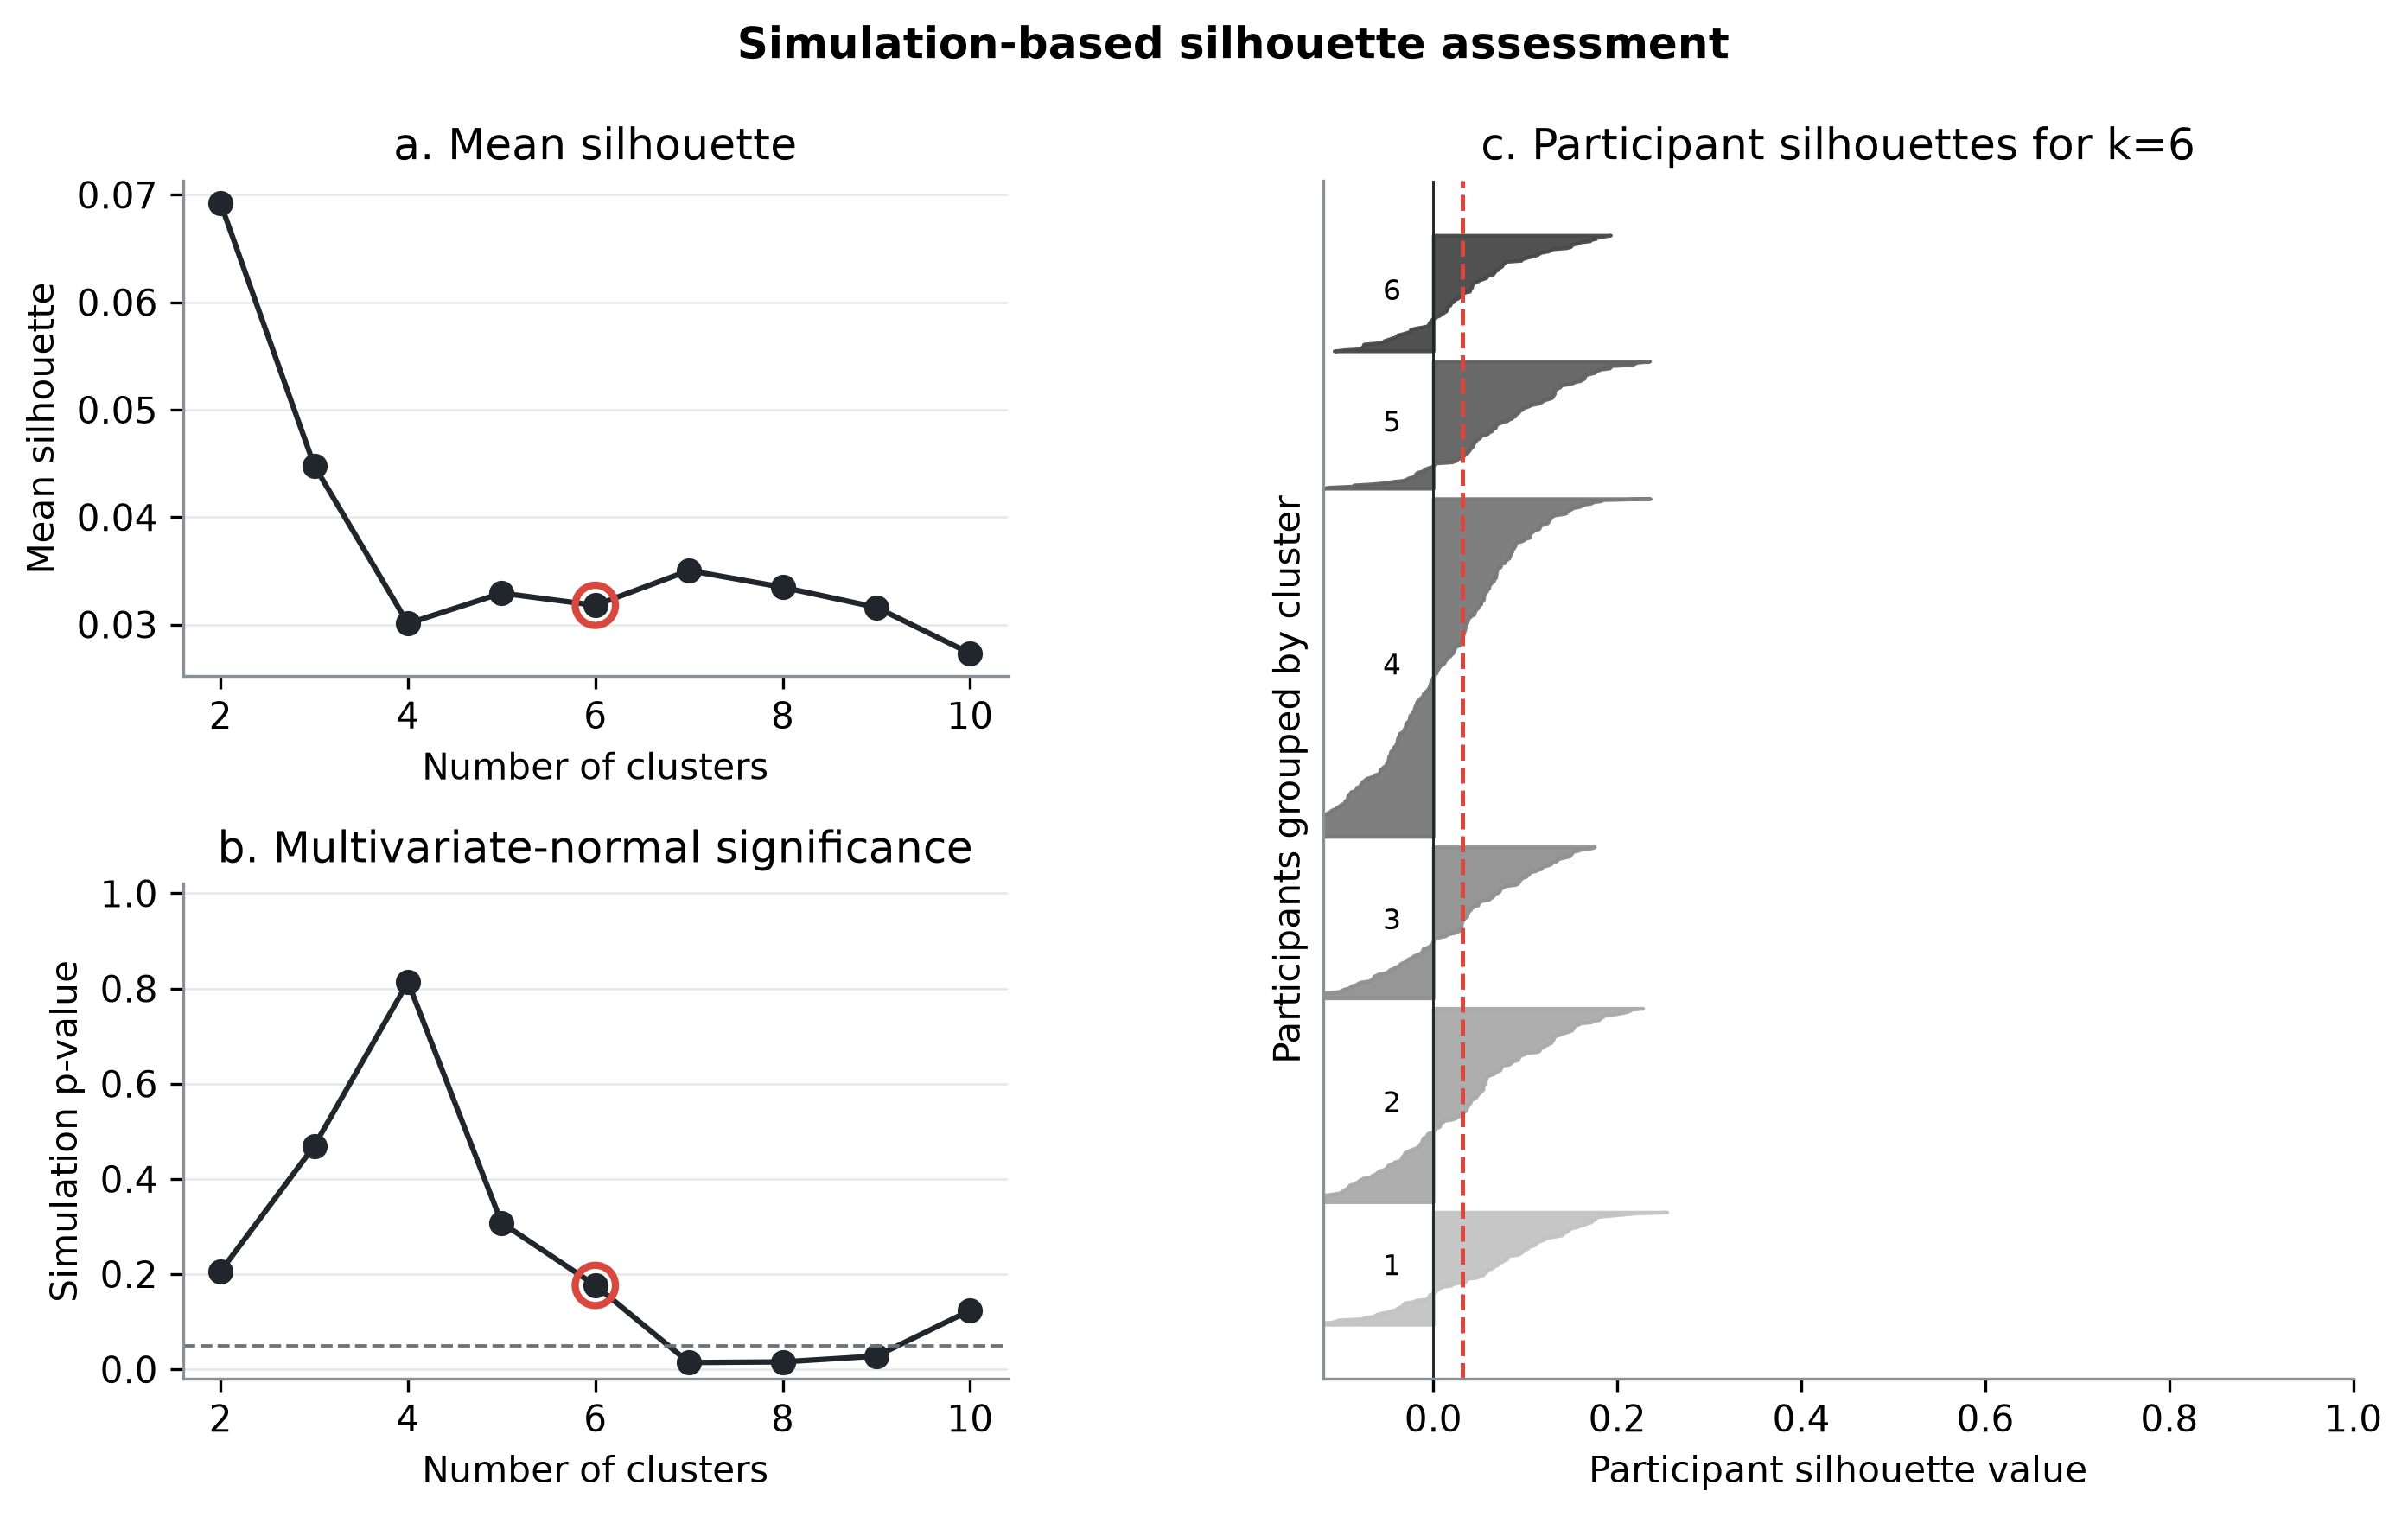
\includegraphics[width=\linewidth,height=.69\textheight,keepaspectratio]{figures/current_silhouette.png}
\end{frame}

\begin{frame}{Profiles: all 31 features, shown in the paper’s visual grammar}
\centering
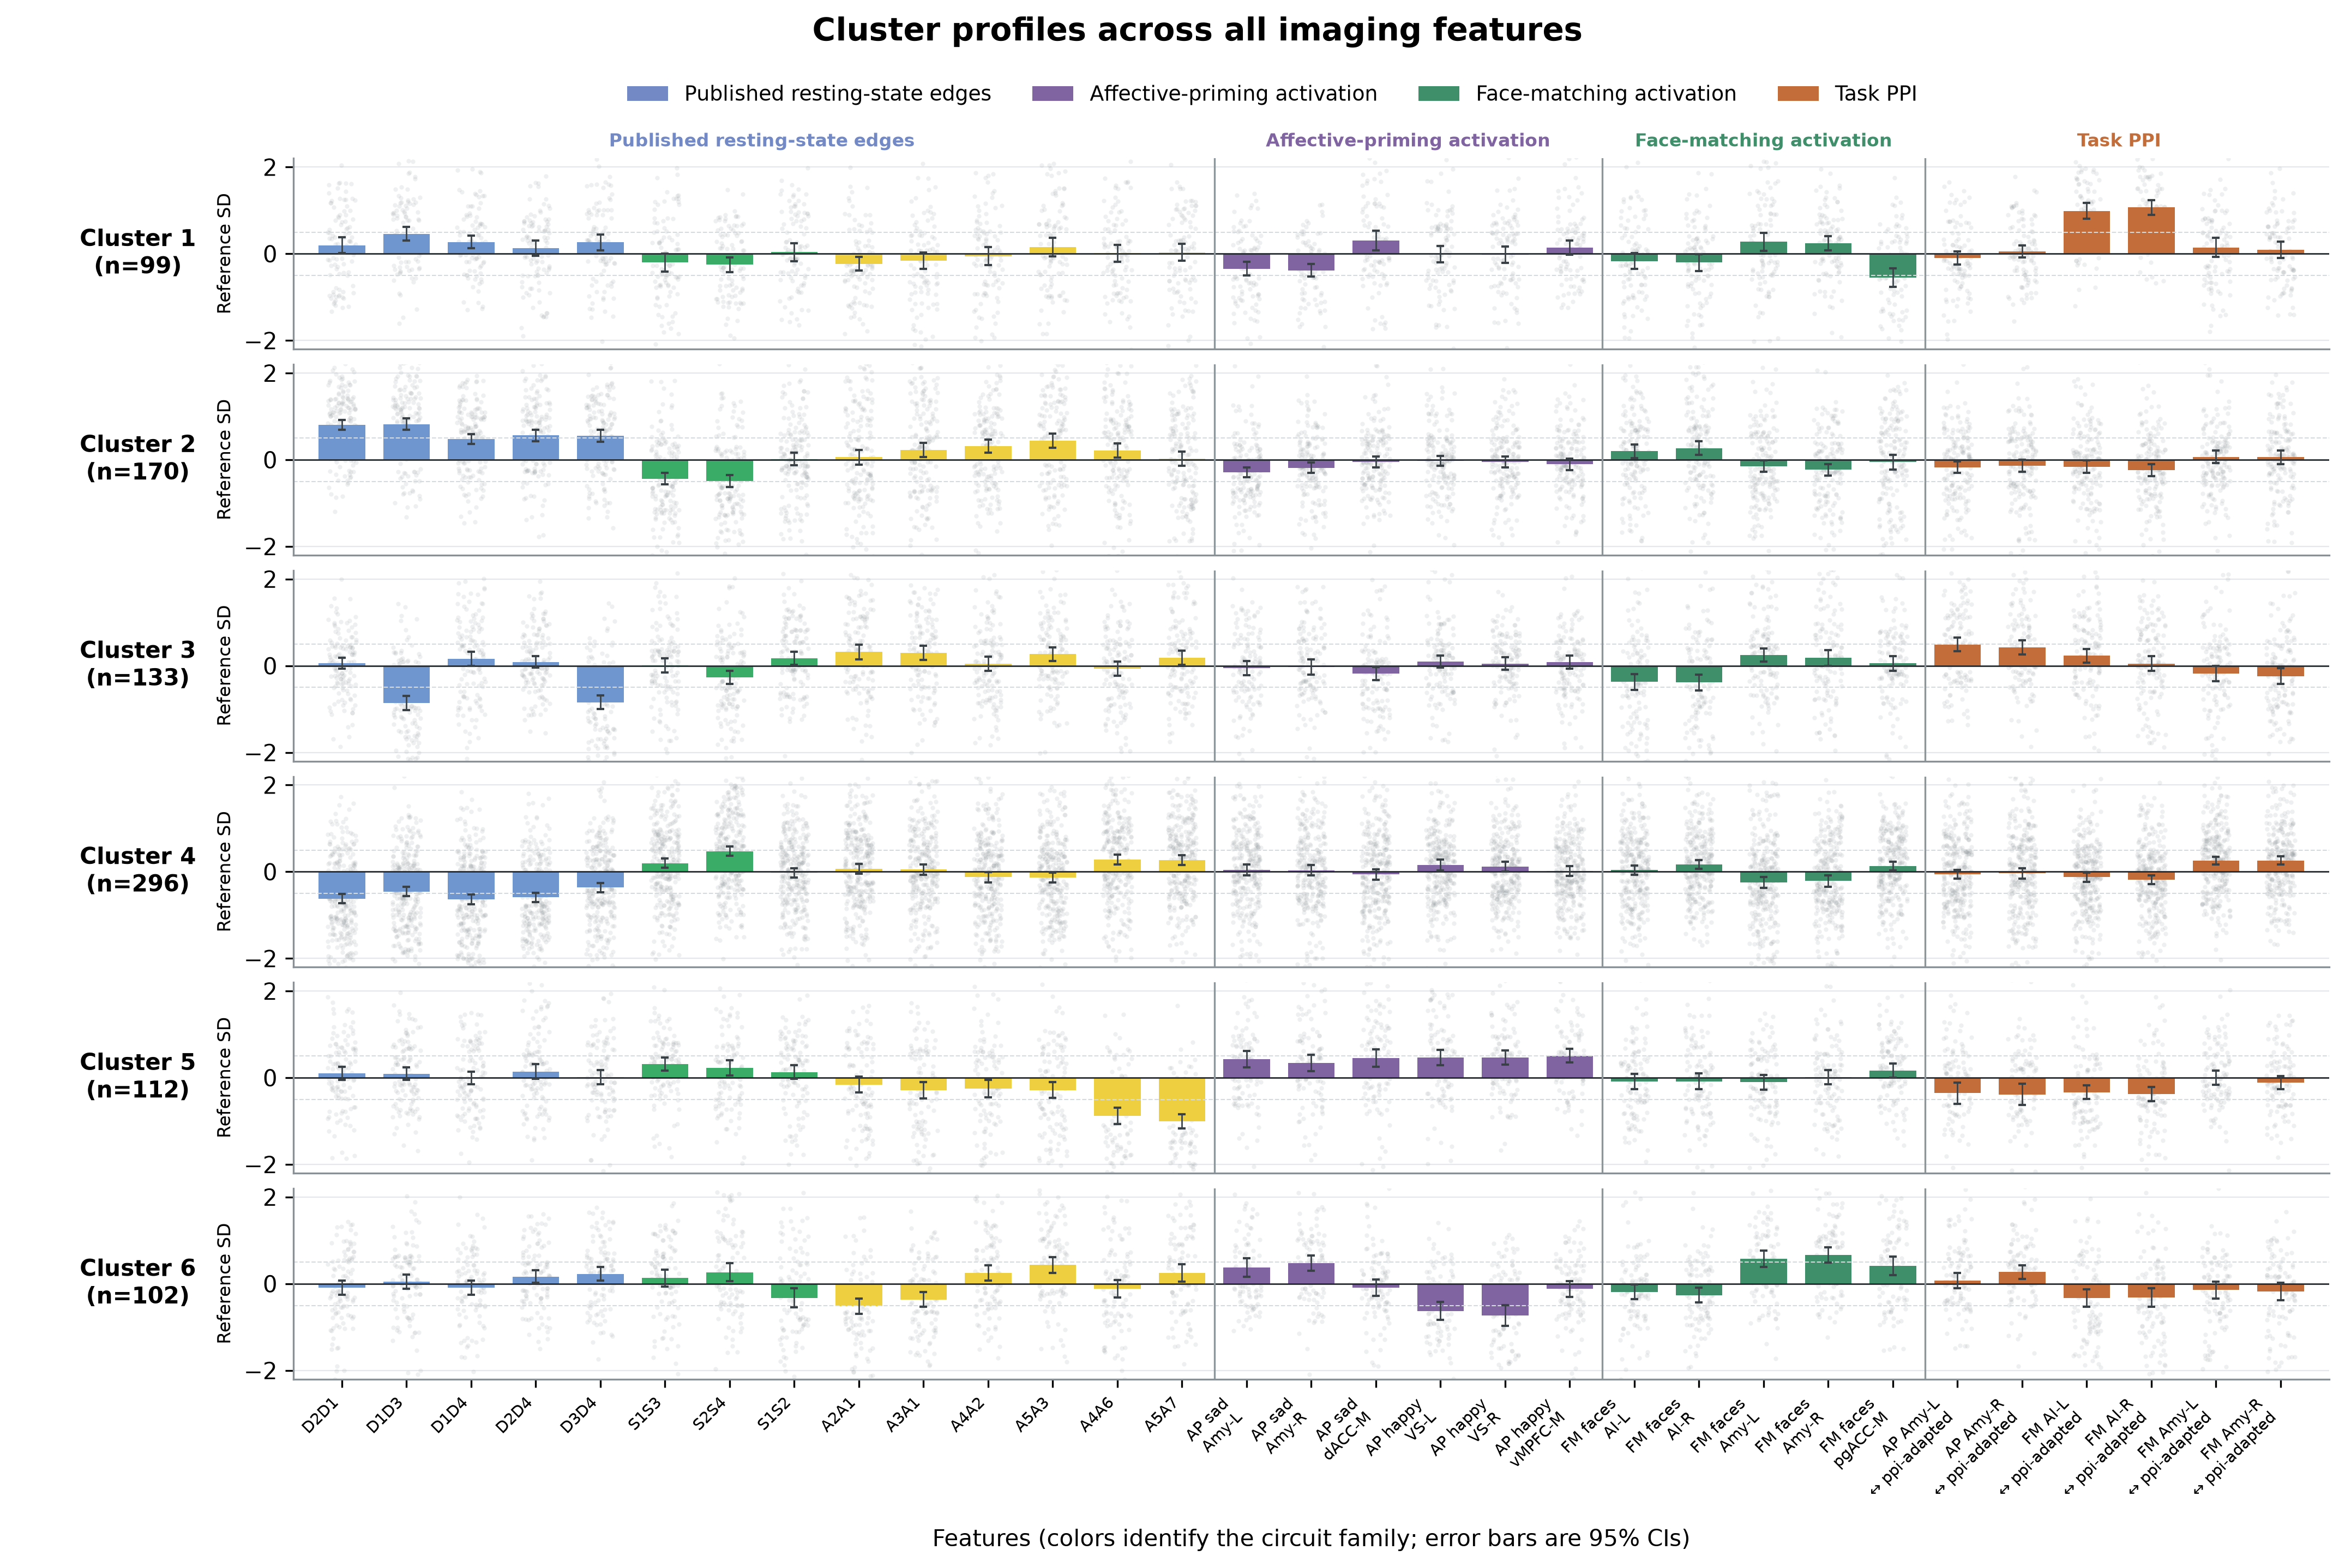
\includegraphics[width=.98\textwidth,height=.77\textheight,keepaspectratio]{figures/current_profiles.png}
\end{frame}

\begin{frame}{Closest FOR2107 matches to Tozzi’s feature set}
\small
\centering
\renewcommand{\arraystretch}{1.28}
\resizebox{\textwidth}{!}{%
\begin{tabular}{@{}p{3.1cm}p{4.0cm}p{4.4cm}r@{}}
\toprule
\textbf{Data source} & \textbf{Task / contrast} & \textbf{Circuit targeted} & \textbf{Features}\\
\midrule
Task-free fMRI & No task; band-limited connectivity & Default mode (5), salience (3), attention (6) & 14\\
Affective-priming task & Sad $>$ neutral & Negative affect — sad analogue (5 activations + 4 PPIs) & 9\\
Affective-priming task & Happy $>$ neutral & Positive affect (3 activations) & 3\\
Threat-face task & No matching FOR2107 contrast & Negative affect — conscious threat & 0\\
Threat-face task & No matching FOR2107 contrast & Negative affect — non-conscious threat & 0\\
Go/NoGo task & No Go/NoGo task available & Cognitive control & 0\\
\midrule
\multicolumn{3}{r}{\textbf{Total closest-match profile}} & \textbf{26}\\
\bottomrule
\end{tabular}}
\vspace{.15cm}
\end{frame}

\begin{frame}
	\frametitle{Discussion}
	\large \centering How should we move forward?
\end{frame}

\end{document}
